\section{Strategia risolutiva e Architettura proposta}
Per risolvere il problema è stato utilizzato un modello ad attori, il quale permette uno scambio di messaggi asincrono tra oggetti reattivi e autonomi che vengono chiamati appunto \textit{attori}.\newline
Ogni entità presente in questo modello deve dunque essere un attore, caratterizzato da un proprio ID univoco e una mailbox che gli permette di accodare i messaggi ricevuti. Gli attori hanno uno stato al quale sono gli unici a poter accedere e per questa ragione ogni interazione deve avvenire tramite lo scambio asincrono di messaggi.

\subsection{Suddivisione delle responsabilità}
Nella soluzione scelta è stato individuato un attore principale denominato \textit{MainActor}, il cui compito è quello di creare il \textit{FileManagerActor} e il \textit{GUIManagerActor} quando riceve il messaggio di inizio dal main. Una volta creati, il \textit{MainActor} comunica a entrambi gli attori di iniziare la computazione.\newline
A questo punto l'elaborazione dei documenti viene svolta dal \textit{FileManagerActor}, il quale crea un numero di \textit{DocumentActors} pari al numero di documenti da computare. In questo modo ogni attore appena creato potrà svolgere in modo indipendente l'elaborazione del documento che gli è stato assegnato e comunicherà con il \textit{FileManagerActor} solo nel momento in cui avrà terminato di contare tutte le parole del file.\newline

\noindent Il \textit{FileManagerActor}, ogni volta che l'elaborazione di un documento è completata, controlla se tutti gli attori figli che ha creato hanno terminato: questo coinciderebbe con la fine di tutta la computazione e porterebbe alla creazione del messaggio con le parole contante e il tempo impiegato. In caso contrario, invia un messaggio al \textit{GUIManagerActor} aggiornando la struttura dati con le nuove informazioni elaborate e continua ad attendere gli altri \textit{DocumentActors}.

\begin{figure}[H]
	\begin{center}
		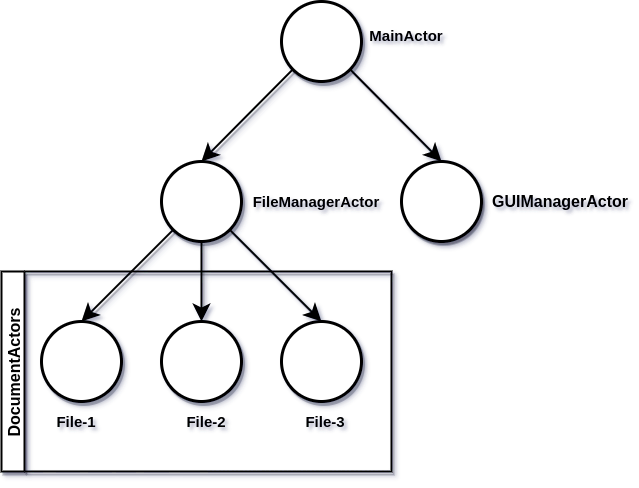
\includegraphics[width=0.8\linewidth]{img/part-1/Actors.png}
	\end{center}
	\caption{Modello ad Attori utilizzato}
\end{figure}

\subsection{Messaggi}

Ogni attore può ricevere diversi tipi di messaggi. Grazie al metodo \textit{receiveBuilder()} richiamabile dentro in metodo \textit{createReceive()} è possibile verificare che tipo messaggio è arrivato in modo da eseguire le operazioni corrette.
Ogni attore può ricevere determinati tipi di messaggio:
\begin{itemize}
    \item \textbf{MainActor}:
        \begin{itemize}
            \item \textbf{\textit{StartComputationMessage}}: Quando arriva un messaggio di questo tipo significa che inizia tutta la computazione. Il MainActor si occupa quindi di creare ed inviare due messaggi:
            \begin{enumerate}
                \item \textit{StartMessage (a FileManagerActor)}: Ordina a FileManagerActor di iniziare la computazione. All'interno del messaggio ci sono tutti gli argomenti (il path della cartella dei documenti, quello del file che contiene le parole da ignorare e il numero di parole da mostrare a fine computazione).
                \item \textit{PrintMessage (a GUIManagerActor)}:
                Ordina a GUIManagerActor di stampare a schermo il messaggio "Computation started!".
            \end{enumerate}
        \end{itemize}
    \item \textbf{FileManagerActor}:
        \begin{itemize}
            \item \textbf{\textit{StartMessage}}: Inizia la computazione, vengono creati tanti attori di tipo \textit{DocumentActor} quanti sono i documenti e viene inviato loro un \textit{BeginComputationMessage}.
            \item \textbf{\textit{StopComputationMessage}}:
            Gli attori figli vengono fermati e deallocati. Viene poi inviato un \textit{PrintMessage} a \textit{GUIManagerActor}, il quale stamperà il messaggio "Computation Stopped".
            \item \textbf{\textit{FinishedComputationMessage}}:
            La computazione di un documento è finita. Viene controllato se sono stati computati tutti i documenti, e nel caso si recuperano i risultati, si ordinano e si manda un \textit{ComputationOverMessage} a \textit{GUIManagerActor}, il quale stamperà i risultati e il tempo impiegato. Altrimenti il FileManagerActor manderà un {PrintMessage} al GUIManagerActor che aggiorna lo stato attuale delle stampe.
        \end{itemize}
    \item \textbf{GUIManagerActor}:
        \begin{itemize}
            \item \textbf{\textit{PrintMessage}}: Il contenuto del messaggio viene stampato sulla GUI.
            \item \textbf{\textit{ComputationOverMessage}}: Stesso funzionamento di \textit{PrintMessage}, ma lo stato della GUI viene anche riportato allo stato iniziale in modo da poter effettuare una nuova computazione.
        \end{itemize}
    \item \textbf{DocumentActor}:
        \begin{itemize}
            \item \textbf{\textit{BeginComputationMessage}}: Il messaggio che inizializza il documento e lo carica in memoria. Vengono estratte tutte le parole e inserite ordinatamente in una lista. Infine invia un messaggio di tipo \textit{ComputeWordMessage} a sé stesso il quale contiene l'indice dell'ultimo elemento della lista.
            \item \textbf{\textit{ComputeWordMessage}}: La parola contenuta nella posizione specificata nell'indice del messaggio viene recuperata e aggiunta al conteggio di una struttura dati interna. Se l'indice è 0 le parole sono finite e viene inviato un \textit{FinishedComputationMessage} all'attore padre. Se l'indice non è uguale a 0 le parole non sono finite e viene inviato un ulteriore \textit{ComputeWordMessage} contenente l'indice decrementato di uno. L'idea è di partire dalla fine della lista e iterare fino al suo inizio.
        \end{itemize}
\end{itemize}
